\section{Mean Value Theorem}
\begin{theorem}
	If $f$ is continuous on the interval $[a,b]$ and differentiable on the interval $(a,b)$, then there exists at least one point in $(a,b)$ such that
	\begin{equation*}
		f^\prime(c) = \frac{f(b)-f(a)}{b-a}.
	\end{equation*}
\end{theorem}
\noindent
That is, there's at least one point where the instantaneous rate of change and average rate of change are equal.
Another way of visualizing this is that there's al least one point where the tangent and secant lines are parallel.

\begin{figure}[H]
	\label{mvt}
	\centering
	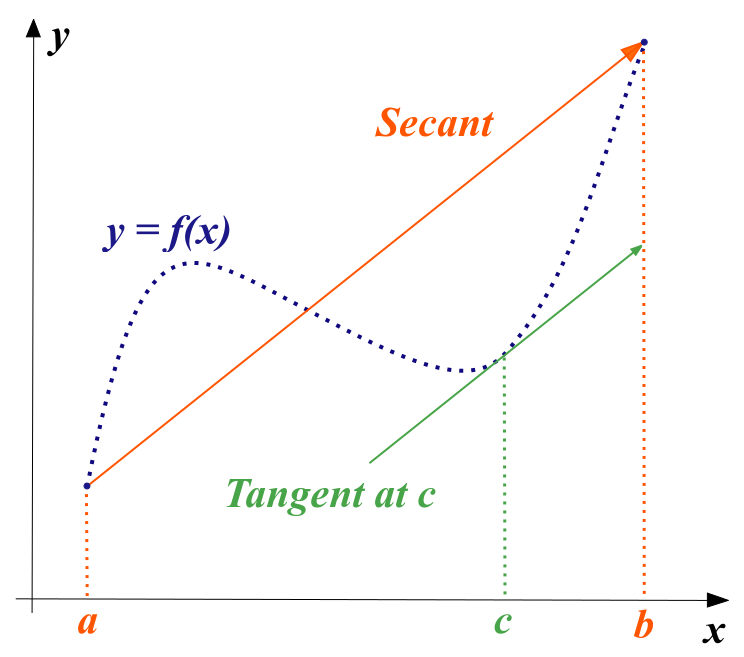
\includegraphics[width = 0.5\textwidth]{./applications_derivative/mvt.png}
	\caption{\hyperref{https://en.wikipedia.org/wiki/Mean\_value\_theorem}{}{}{Wikipedia - Mean Value Theorem}}
\end{figure}

\begin{example}
	A trucker drives 150 miles of a route in 2 hours.
	The speed limit along the route is 65 miles per hour.
	Show that at at least one point, the trucker must have been speeding.
\end{example}
We can model the trucker's position along the route $s$ as a function of time $t$ where $s(0)=0$ and $s(2)=150$.
We know that velocity is the derivative of position, so $v(t) = s^\prime(t)$.
It's reasonable to assume that $s$ is differentiable on the interval $[0,2]$.
So, by the Mean Value Theorem, there must exist a point $c$ where
\begin{equation*}
	v(t) = \frac{s(2)-s(0)}{2-0} = \frac{150-0}{2} = 75\text{mph}.
\end{equation*}
\indent
At this point, the trucker was exceeding the speed limit of 65 miles per hour.

\begin{definition}
	Let $f$ be defined on an interval $I$.
	Let $a$ and $b$ be any two different points in $I$.
	\begin{align*}
		\text{$f$ increases on $I$ if } a < b &\implies f(a) < f(b). \\
		\text{$f$ decreases on $I$ if } a < b &\implies f(a) > f(b).
	\end{align*}
\end{definition}

\begin{corollary}
	Let $f$ be continuous of $[a,b]$ and differentiable on $(a,b)$.
	\begin{align*}
		\text{If $f^\prime > 0$ at every point on $(a,b)$ then $f$ increases on $[a,b]$}. \\
		\text{If $f^\prime < 0$ at every point on $(a,b)$ then $f$ decreases on $[a,b]$}.
	\end{align*}
\end{corollary}
\noindent
This should make sense given our theorem about local extrema.
If $f$ could still increase/decrease while its derivative was negative/positive, then we couldn't be sure that $f$ is at a local maxima/minima when $f^\prime=0$.

\begin{corollary}
	If $f^\prime(x) = 0$ at all points in an interval $I$, then there is some constant $C$ such that $f(x) = C$ for all points in $I$.
\end{corollary}
\noindent
This follows from the Mean Value Theorem.
Since $f^\prime = 0$, the numerator in the Mean Value Theorem, $f(b) - f(a)$, must also be 0, meaning $f(b) = f(a) = C$.

\begin{corollary}
	If $f^\prime(x) = g^\prime(x)$ at ever point in some interval $I$, then there is come constant $C$ such that $f(x) = g(x) + C$.
\end{corollary}
\noindent
That is, functions with the same derivative differ by a constant.
This should make sense given our constant and sum and difference derivative rules.
If we let $h^\prime(x) = f^\prime(x) - g^\prime(x) = 0$ and apply the previous corollary, we get $C$.

\begin{definition}
	A function $F(x)$ is the antiderivative	of $f(x)$ if $F^\prime(x) = f(x)$ for all points in the domain of $f$.
\end{definition}
\noindent
As we saw in the previous corollary, a function will have infinitely many antiderivatives that differ by a constant.